\usetikzlibrary{positioning}

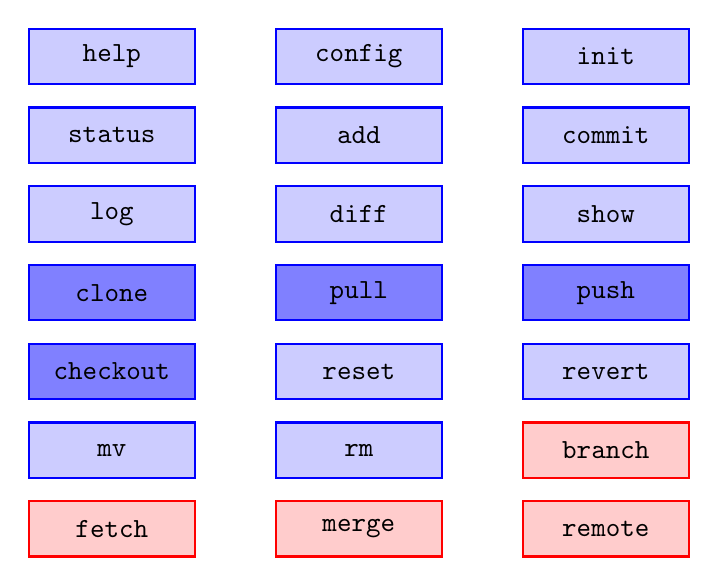
\begin{tikzpicture}
[
gitcommand/.style={rectangle, minimum width=6em, minimum height=2em, 
fill=blue!20, 
draw=blue, thick},
newgitcommand/.style={rectangle, minimum width=6em, minimum height=2em, 
fill=red!20, 
draw=red, thick},
todaygitcommand/.style={rectangle, minimum width=6em, minimum height=2em, 
fill=blue!50, 
draw=blue, thick},
]

\node [gitcommand] (config) at (0,0) {\texttt{config}};
\node [gitcommand, left = of config] (help) {\texttt{help}};
\node [gitcommand, right = of config] (init) {\texttt{init}};
\node [gitcommand, below of = help] (status) {\texttt{status}};
\node [gitcommand, below of = config] (add) {\texttt{add}};
\node [gitcommand, below of = init] (commit) {\texttt{commit}};
\node [gitcommand, below of = status] (log) {\texttt{log}};
\node [gitcommand, below of = add] (diff) {\texttt{diff}};
\node [gitcommand, below of = commit] (show) {\texttt{show}};
\node [todaygitcommand, below of = log] (clone) {\texttt{clone}};
\node [todaygitcommand, below of = diff] (pull) {\texttt{pull}};
\node [todaygitcommand, below of = show] (push) {\texttt{push}};
\node [todaygitcommand, below of = clone] (checkout) {\texttt{checkout}};
\node [gitcommand, below of = pull] (reset) {\texttt{reset}};
\node [gitcommand, below of = push] (revert) {\texttt{revert}};
\node [gitcommand, below of = checkout] (mv) {\texttt{mv}};
\node [gitcommand, below of = reset] (rm) {\texttt{rm}};
\node [newgitcommand, below of = revert] (branch) {\texttt{branch}};
\node [newgitcommand, below of = mv] (fetch) {\texttt{fetch}};
\node [newgitcommand, below of = rm] (merge) {\texttt{merge}};
\node [newgitcommand, below of = branch] (remote) {\texttt{remote}};

%  \item \texttt{clone}

\end{tikzpicture}
